\documentclass[spanish]{beamer}
\usepackage[ansinew]{inputenc} % Acepta caracteres en castellano
\usepackage[spanish]{babel}    % silabea palabras castellanas
\usepackage{amsmath}
\usepackage{mathtools,cancel} % cancela con una flecha \cancelto{0}{XXXX}
\renewcommand{\CancelColor}{\color{red}} %change cancel color to red
\usepackage{amsfonts}
\usepackage{amssymb}
\usepackage{dsfont}
\usepackage{graphicx}
\usepackage{geometry}
\usetheme{Madrid}
\usecolortheme{beaver}
\usepackage{textpos}
% Logo  en el comienzo 
\addtobeamertemplate{frametitle}{}{%
\begin{textblock*}{100mm}(.85\textwidth,-1cm)
{\includegraphics[height=0.4in, keepaspectratio=true]{/Users/luisnunez/Dropbox/MisDocumentos/UIS/UISImagenInstitucional/UISLOGO.png}}
\end{textblock*}}

\begin{document}

\title{\textbf{Dos Problemas S�lidos} }
\author[L.A. N��ez]{\textbf{Luis A. N��ez}}  
\institute[UIS]{\textit{Escuela de F�sica, Facultad de Ciencias, } \\
\textit{Universidad Industrial de Santander, Santander, Colombia } \\
{\includegraphics[height=0.4in, keepaspectratio=true]{/Users/luisnunez/Dropbox/MisDocumentos/UIS/UISImagenInstitucional/UISLOGO.png}}
}
\date{\today}
\maketitle


\begin{frame}
\frametitle{Agenda}
  \tableofcontents
\end{frame}


%%%%% Diapo 1
\section{Moneda que rueda sin deslizar}
\subsection{Ligaduras}
\frame{
  \frametitle{Moneda que rueda sin deslizar: Ligaduras}
Un disco homog�neo (una moneda) de radio $a$ y masa $M$ rueda sin deslizar por una superficie plana. Escriba las ecuaciones de movimiento y encuentre una soluci�n en el caso en que la inclinaci�n del disco sea constante.
\begin{figure}[t]
	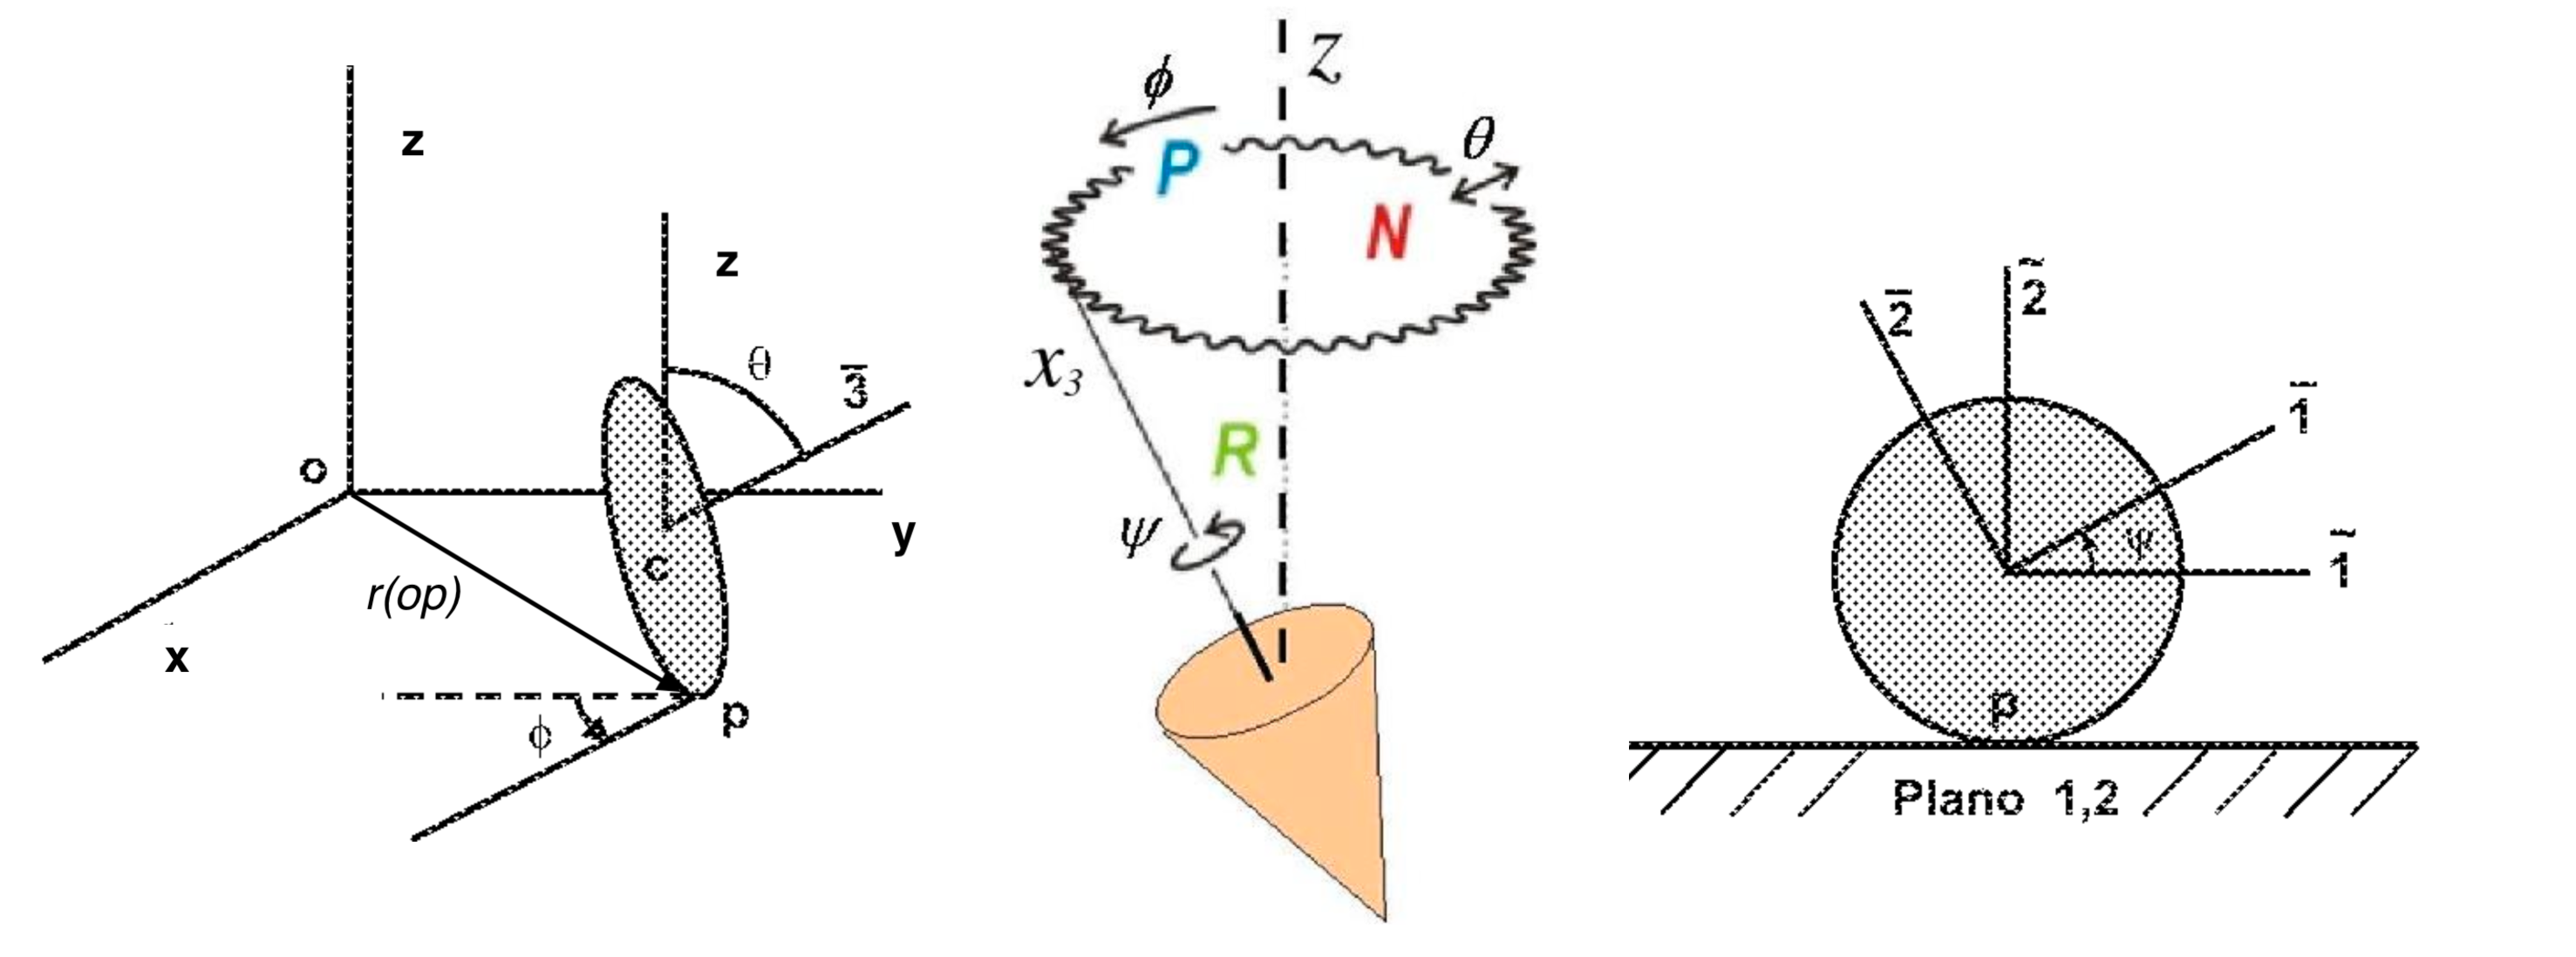
\includegraphics[width=2.8in]{Figuras/Moneda.pdf}
\end{figure}
   \begin{itemize}  
  	\item<1-> En principio tendremos seis grados de libertad $(x, y, z, \phi, \psi, \theta)$: \\ tres de traslaci�n y tres �ngulos de Euler. 
	\item<3->  La ligadura de rodar sin deslizar implica que la velocidad del punto $p$, en contacto con la superficie, es instant�neamente cero.
	\item<4-> Esto es: $\vec{r}(op)=\vec{R}+\vec{r}(cp) \Rightarrow \dot{\vec{r}}(op)_{p}=0=\dot{\vec{R}}+  \vec{\Omega} \times \vec{r}(cp)$ 
    \end{itemize}
}
%%%%% Diapo 2
\subsection{El Lagrangeano}
\frame{
\frametitle{Moneda que rueda sin deslizar: Lagrangeano}
\begin{itemize}
	\item<1-> Por su parte, respecto al sistema centro de masa, $\tilde{S}$ tenemos $\vec{r}(cp) = -a {\bf \hat{x}}^2$, y $\vec{\Omega} \times \vec{r}(cp) = 
	\left|
	\begin{array}{ccc} 
	{\bf \hat{x}}^1 & {\bf \hat{x}}^2 & {\bf \hat{x}}^3 \\
	\tilde{\Omega}^1 & \tilde{\Omega}^2 & \Omega^3 \\
	0 & -a & 0
	\end{array}\right| = a(\Omega^3 \, {\bf \hat{x}}_1 -\Omega^1\, {\bf \hat{x}}_3) $
	\item<2-> Respecto al sistema centro de masa 
	$\Omega_1  = \dot{\phi} \operatorname{sen} \, \theta \operatorname{sen} \, \psi+\dot{\theta} \cos \psi $ \\
	$\Omega_2  = \dot{\phi} \operatorname{sen} \, \theta \cos \psi-\dot{\theta} \operatorname{sen} \, \psi \quad $  y 
	$\quad \Omega_3  = \dot{\psi}+\dot{\phi} \cos \theta$
	\item<2-> Proyectamos la ecuaci�n $0=\dot{\vec{R}}+  \vec{\Omega} \times \vec{r}(cp)$ al sistema $S$, (${\bf i}$, ${\bf j}$, ${\bf k}$) tendremos 
	$\dot{x} + a(\Omega_3 \, {\bf i} \cdot {\bf \hat{x}}_1 -\Omega_1\, {\bf i} \cdot {\bf \hat{x}}_3) = 0 $ \\
	$\dot{y} + a(\Omega_3 \, {\bf j} \cdot {\bf \hat{x}}_1 -\Omega_1\, {\bf j} \cdot {\bf \hat{x}}_3) = 0 $ \\
	$\dot{z} + a(\Omega_3 \, {\bf k} \cdot {\bf \hat{x}}_1 -\Omega_1\, {\bf k} \cdot {\bf \hat{x}}_3) = 0 $
\end{itemize} 
}
%%%%% Diapo 2
\subsection{Secci�n}
\frame{
\frametitle{T�tulo transparencia}
\begin{itemize}
	\item<1-> La energ�a cin�tica ser� $\left.T=\frac{1}{2} M\left(\dot{x}^2+\dot{y}^2+\dot{z}^2\right)+\frac{1}{2}\left[I_{1}(c)\left(\Omega_{1}\right)^2+I_{2}(c)\left(\Omega_{2}\right)^2+I_{3}(c) \Omega_{3}\right)^2\right]$.  
	\item<2-> 	$T=\frac{1}{2} M\left(\dot{x}^2+\dot{y}^2+\dot{z}^2\right)+\frac{1}{8} M a^2\left[\dot{\phi}^2 \operatorname{sen}^2 \theta+\dot{\theta}^2+2\left(\dot{\phi} \cos \theta^2+\dot{\psi}\right)^2\right]$
	\item<2-> Donde $I_{1}=I_{2}=M a^2 / 4$ y $I_{3}=M a^2 / 2$.
	\item<3-> Por su parte, la energ�a potencial $V = mga \operatorname{sen} \theta$
	\item<4-> El Lagrangeano $\mathcal{L} = T-V$, $\mathcal{L} = \frac{1}{2} M\left(\dot{x}^2+\dot{y}^2+\dot{z}^2\right)+\frac{1}{8} M a^2\left[\dot{\phi}^2 \operatorname{sen}^2 \theta+\dot{\theta}^2+2\left(\dot{\phi} \cos \theta^2+\dot{\psi}\right)^2\right] - mga \operatorname{sen} \theta$

\end{itemize}
}
%%%%% Diapo 2
\section{Moneda en un plano inclinado}
\subsection{Planteamiento del problema}
\frame{
\frametitle{Planteamiento del problema}
Un disco delgado, uniforme, de masa $M$ y radio a est� enganchado a una varilla $A C$ sin masa de longitud $b$. El sistema est� en un plano inclinado perfectamente rugoso que forma un �ngulo $\alpha$ con la horizontal. El punto $A$ de la varilla se mantiene fijo en un punto $O$ del plano inclinado mientras que el disco puede rodar libremente sin deslizar. Tomamos como sistema $S$ uno con origen en $O$, eje $z$ perpendicular al plano inclinado y el eje $y$ hacia arriba del plano y para el sistema $\tilde{S}$ origen tambi�n en $O$ y eje $\tilde{3}$ en la direci�n $A C$. Encontrar las ecuaciones de movimiento para 
\begin{itemize}
	\item $\alpha = 0$
	\item $\alpha \neq 0$
\end{itemize}
\begin{figure}[t]
	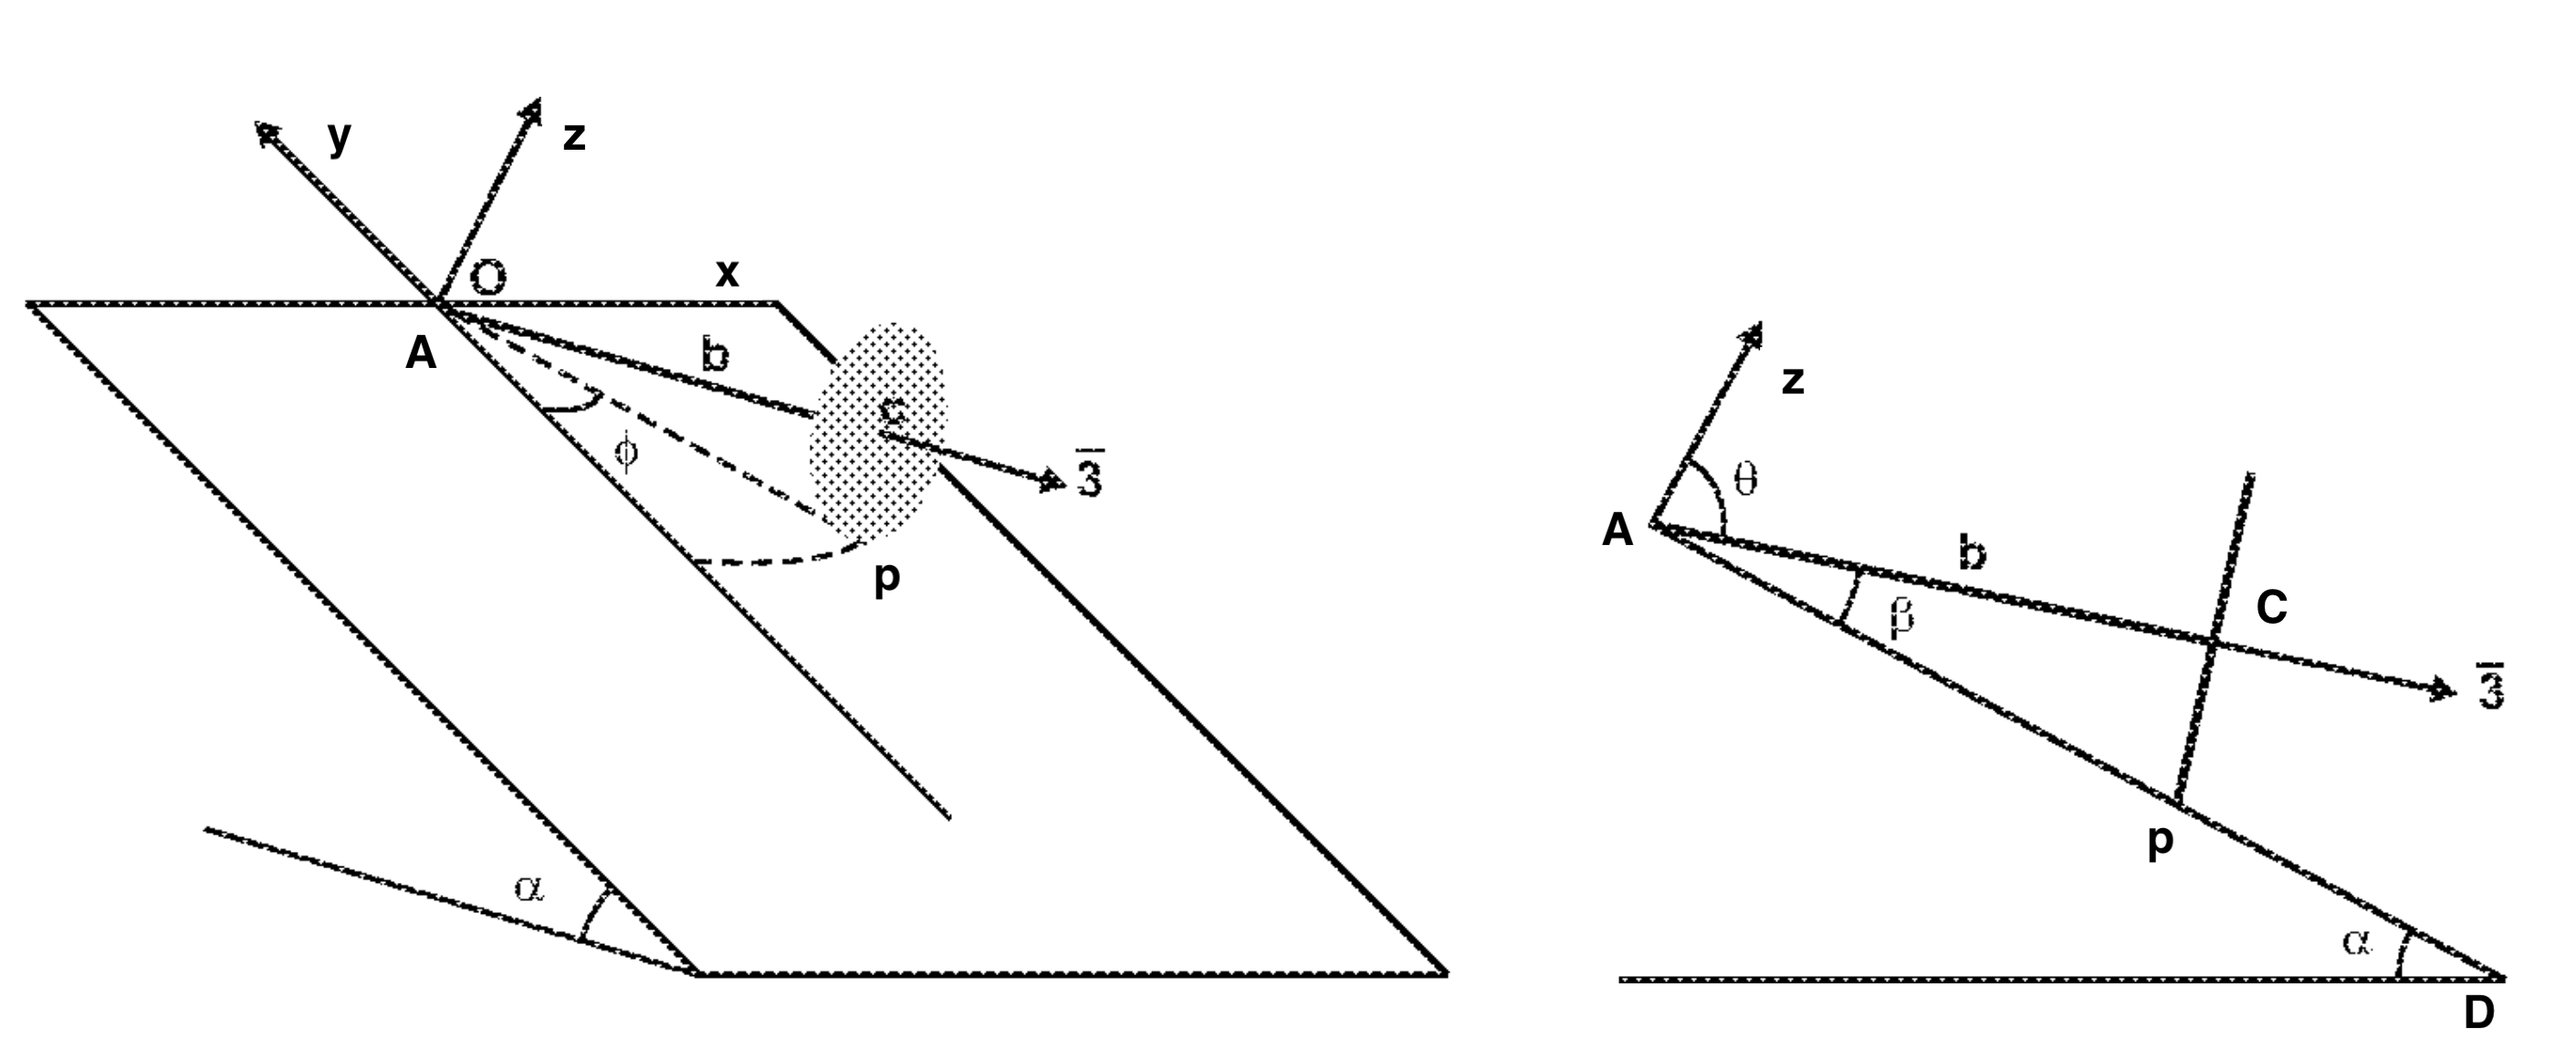
\includegraphics[width=3.0in]{Figuras/MonedaInclinada.png}
\end{figure}
}
%%%%% Diapo 2
\subsection{Coordenadas y ligaduras}
\frame{
\frametitle{Coordenadas y ligaduras}
\begin{itemize}  
	\item<1-> En principio tenemos seis grados de libertad $(x, y, z, \phi, \psi, \theta)$ y cinco ligaduras
	\item<2-> $\theta=$ constante implica  $\theta+\beta=\frac{\pi}{2}, \quad \tan \beta=\frac{a}{b}, \quad \theta=\frac{\pi}{2}-\arctan \frac{a}{b}$
	\item<3-> $|{\bf R}| = b$. M�s a�n, ${\bf R} =b {\bf \hat{x}}_3= b\left[\operatorname{sen} \phi \operatorname{sen} \theta {\bf \hat{x}}-\cos \phi \operatorname{sen} \theta {\bf \hat{y}}+\cos \theta {\bf \hat{z}}\right]$,
	\item<4-> Entonces $x = b\operatorname{sen} \phi \operatorname{sen} \theta $; $\quad y =-b\cos \phi \operatorname{sen} \theta \quad$ y $z = b\cos \theta $ que cumplen con la ecuaci�n $x^2 +y^2 +z^2 = b^2$
	\item<5-> Deriv�ndolas con $\theta=$ const., se obtiene: $
\dot{x}=b \dot{\phi} \cos \phi \operatorname{sen} \theta, \quad \dot{y}=b \dot{\phi} \operatorname{sen} \phi \operatorname{sen} \theta, \quad \dot{z}=0$
	\item<6-> Rodar sin deslizar implica que la velocidad del punto $p$ es cero : ${\bf r}_{op}={\bf R}+{\bf r}_{cp} \Rightarrow \dot{{\bf r}}_{op} = 0=\dot{{\bf R}}+  \tilde{ {\bf \Omega}} \times {\bf r}_{cp}$.
	\item<7-> Respecto al sistema centro de masa, $\tilde{S}$ tenemos ${\bf r}_{cp} = -a {\bf \hat{x}}_2$, y $\tilde{{\bf \Omega}} \times {\bf r}_{cp} = 
	\left|
	\begin{array}{ccc} 
	{\bf \hat{x}}_1 & {\bf \hat{x}}_2 & {\bf \hat{x}}_3 \\
	\tilde{\Omega}^1 & \tilde{\Omega}^2 & {\tilde \Omega}^3 \\
	0 & -a & 0
	\end{array}\right| = a(\tilde{\Omega}^3 \, {\bf \hat{x}}_1 -\tilde{\Omega}^1\, {\bf \hat{x}}_3) $
	con cual respecto al centro de masa $b \dot{{\bf \hat{x}}}_3 +a(\tilde{\Omega}^3 \, {\bf \hat{x}}_1 -\tilde{\Omega}^1\, {\bf \hat{x}}_3) =0$

\end{itemize}
}

\section{Secci�n}
\frame{
\frametitle{T�tulo transparencia}
\begin{itemize}
	\item<1-> Al proyectar la ecuaci�n de ligadura $0=\dot{{\bf R}}+ a(\tilde{\Omega}^3 \, {\bf \hat{x}}_1 -\tilde{\Omega}^1\, {\bf \hat{x}}_3) $ 
	respecto a la base del Sistema laboratorio tendremos \\
	$\dot{x} + a(\tilde{\Omega}^3 ({\bf \hat{x}} \cdot {\bf \hat{x}}_1) -\tilde{\Omega}^1 ({\bf \hat{x}} \cdot {\bf \hat{x}}_3))=0 $; $\quad \dot{y} + a(\tilde{\Omega}^3  ({\bf \hat{y}} \cdot {\bf \hat{x}}_1) -\tilde{\Omega}^1 ({\bf \hat{y}} \cdot {\bf \hat{x}}_3)) =0$; $\quad \dot{z} + a(\tilde{\Omega}^3  ({\bf \hat{z}} \cdot {\bf \hat{x}}_1) -\tilde{\Omega}^1 ({\bf \hat{z}} \cdot {\bf \hat{x}}_3)) =0 $.
	\item<2-> que se convierte en 
	$ \dot{x}+a(\dot{\psi} \cos \phi+\dot{\phi} \cos \phi \cos \theta-\dot{\theta} \operatorname{sen} \phi \operatorname{sen} \theta)=0$ \\
	$ \dot{y}+a(\dot{\psi} \operatorname{sen} \phi+\dot{\phi} \operatorname{sen} \phi \cos \theta+\dot{\theta} \cos \phi \operatorname{sen} \theta)=0$ \\
	$ \dot{z}-a \dot{\theta} \cos \theta=0 $
	\item<3-> y usando las otras ecuaciones de ligadura $\dot{x}=b \dot{\phi} \cos \phi \operatorname{sen} \theta, \quad \dot{y}=b \dot{\phi} \operatorname{sen} \phi \operatorname{sen} \theta, \quad \dot{z}=0$, obtenemos $\dot{\psi}+\dot{\phi}\left[\frac{b}{a} \operatorname{sen} \theta+\cos \theta\right]=0 \Rightarrow \psi=-\frac{\sqrt{a^2+b^2}}{a} \phi$
	\item<4-> Donde hemos sustituido el valor de $\theta$ que implica $\operatorname{sen} \theta=b / \sqrt{a^2+b^2}$ y $\cos \theta=a / \sqrt{a^2+b^2}$.
\end{itemize}
}
%%%%% Diapo 2
\subsection{Energ�as Cin�tica, Potencial y el Lagrangeano}
\frame{
\frametitle{Energ�as Cin�tica, Potencial y el Lagrangeano}
\begin{itemize}  
	\item<1-> Como siempre la energ�a cin�tica se construye como 
	$T= T_{tras} + T_{rot} = \frac{1}{2} M(\dot{x}^2+\dot{y}^2+\dot{z}^2)
	+\frac{1}{2}( I_{11} \tilde{\Omega}_1^2 +I_{22} \tilde{\Omega}_2^2 +I_{33} \tilde{\Omega}_3^2 )$
	\item<2-> Los momentos de inercia son: $I_{11} = I_{22}=\frac{1}{4} M a^2$ y $I_{33}=\frac{1}{2} M a^2$.
	\item<3-> Las componentes de la velocidad angular son 
	$\tilde{\Omega}_1  = \dot{\phi} \operatorname{sen} \, \theta \operatorname{sen} \, \psi+\dot{\theta} \cos \psi$; 
	$\quad \tilde{\Omega}_2  = \dot{\phi} \operatorname{sen} \, \theta \cos \psi-\dot{\theta} \operatorname{sen} \, \psi$; 
	$\quad \tilde{\Omega}_3  = \dot{\psi}+\dot{\phi} \cos \theta$.
	\item<4-> Finalmente la energ�a cin�tica queda como $T=\frac{M}{8} \frac{a^2 b^2+6 b^4}{a^2+b^2} \dot{\phi}^2$.
	\item<5-> Para $\alpha = 0$ la energ�a potencial ser� $Mg \frac{ba}{\sqrt{a^2 + b^2}}$

\end{itemize}
}
 
\end{document}


	\item<3->  La ligadura de rodar sin deslizar implica que la velocidad del punto $p$, en contacto con la superficie, es instant�neamente cero.
	\item<4-> Esto es: $\vec{r}(op)=\vec{R}+\vec{r}(cp) \Rightarrow \dot{\vec{r}}(op) = 0=\dot{\vec{R}}+  \vec{\Omega} \times \vec{r}(cp)$

%%%%% Diapo 2
\section{Secci�n}
\frame{
\frametitle{T�tulo transparencia}
\begin{itemize}  
	\item<1-> 
\end{itemize}
}
	\item<2->Las tres primeras components con las coordenadas cartesianas del centro $c$ y las siguientes los �ngulos de Euler. Adem�s $\vec{r}(c p)=-a {\bf k}}$.

	\begin{figure}[t]
		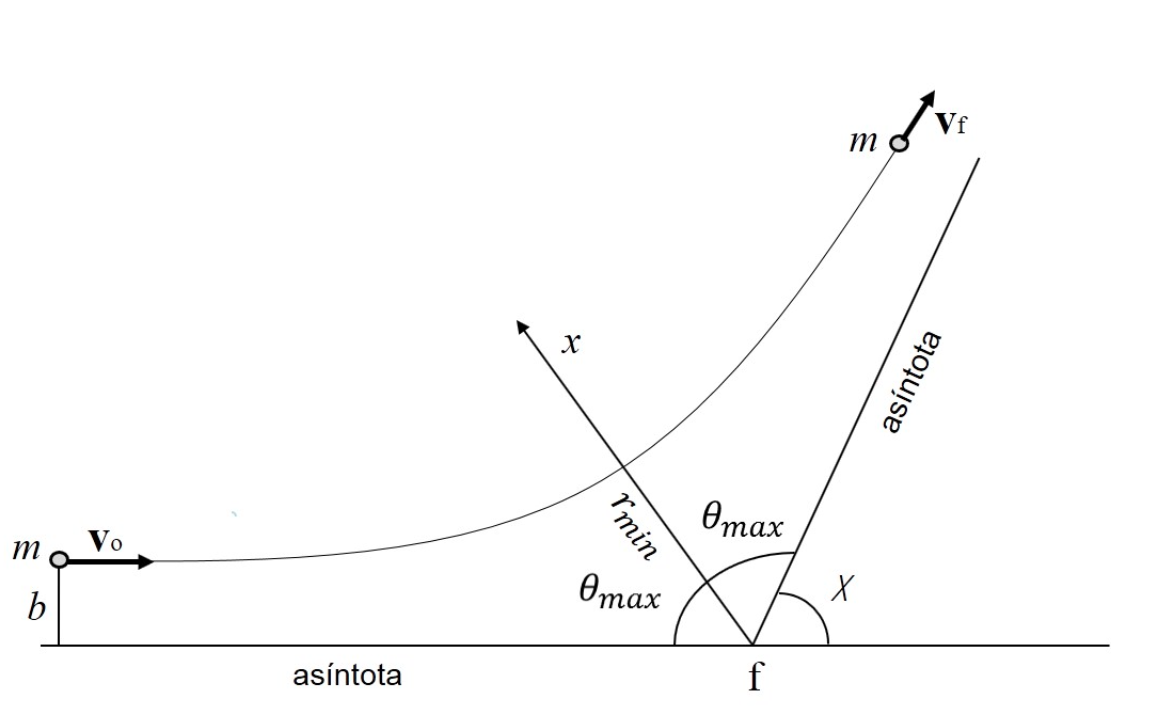
\includegraphics[width=1.8in]{Figuras/Dispersion.png}
   	\end{figure}
	
